
\section{Introduction}
\label{sec:introduction}

\begin{figure}[t]
    \centering
    \par\vspace{-0pt}\par
    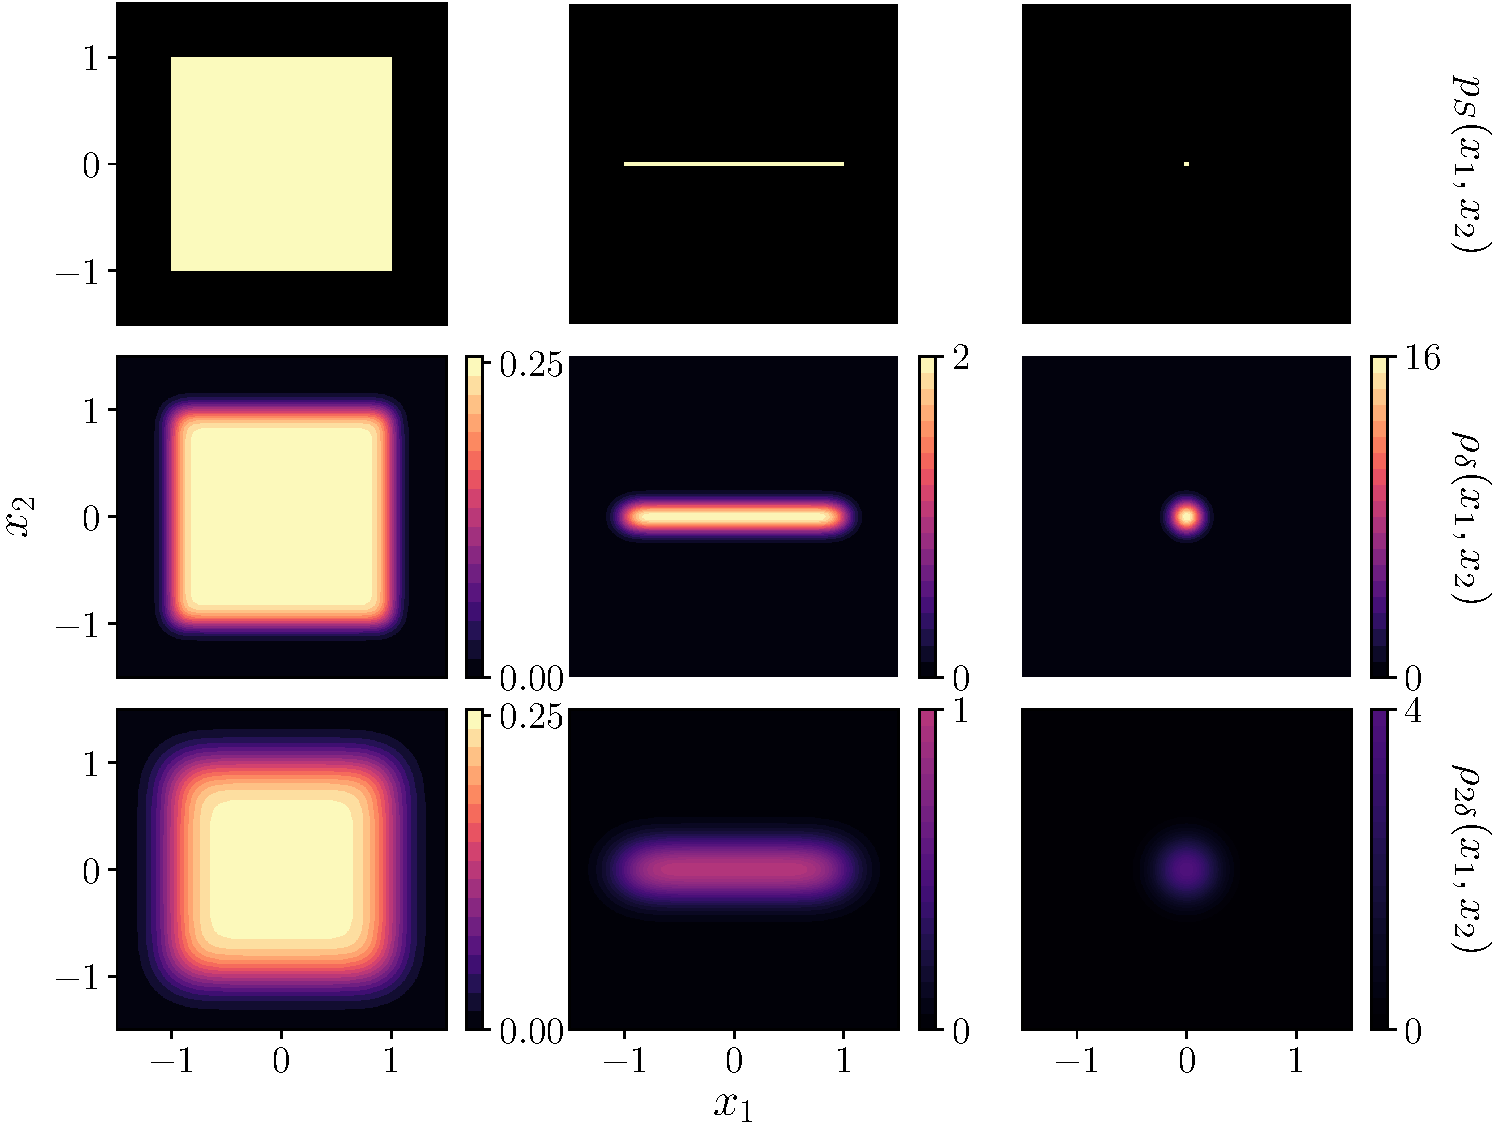
\includegraphics[trim=0 0 0pt 0,clip,width=\linewidth]{images/LIDL_fig_method_6}
    \caption{Illustration of LIDL's core insight. [Top] Three uniform distributions $p_S$ supported respectively on a square, interval, and a point, with intrinsic dimensions $2$, $1$, $0$. 
    [Middle/bottom] Perturbed densities $\rho_{\delta}$ and $\rho_{2\delta}$ resulting from addition of Gaussian noise with different noise magnitudes: $\delta$ and $2\delta$. 
    Our core insight is that the difference between the densities $\rho_{\delta}(x)$ and $\rho_{2\delta}(x)$ at any point $x$ depends on the local intrinsic dimension (LID) at that point. Consider point $x\!=\!(0,0)$. For the left column, that difference is zero; for the middle one, the density is halved; for the right one, it is quartered. We leverage this mechanism to estimate LID.}
    \label{fig:method-1}
\end{figure}



In this paper, we consider the  problem  of local intrinsic dimension (LID) estimation of a lower-dimensional data manifold embedded in a higher-dimensional ambient space. 


Intrinsic dimension estimation is an established problem in data analysis and representation learning \citep{ansuini2019intrinsic,li2018measuring,rubenstein2018latent}.
It was studied in the context of dimensionality reduction, clustering, and classification problems \citep{vapnik2013nature,kleindessner2015dimensionality,camastra2016intrinsic} and
some prototype-based clustering algorithms \citep{claussen2005magnification,struski2018lossy}, among others. 
It is also a powerful analytical tool to study the process of training and representation learning in deep neural networks \citep{li2018measuring, ansuini2019intrinsic}.
\citet{rubenstein2018latent} shows how the mismatch between the latent space dimensionality and the dataset's ID may hurt the performance of auto-encoder generative models like VAE~\citep{kingma2014auto}, WAE \citep{tolstikhin2017wasserstein}, or CWAE \citep{knop2020cramer}.
Recent results of \citet{pope2020intrinsic} show that the global ID of the dataset impacts the training process of a machine learning model, sample efficiency, and its ability to generalize. 

Recently, there has also been a rise of interest in methods for simultaneous manifold learning and density estimation \citep{brehmer2020flowsa,caterini2021rectangular,ross2021tractable}.
Most of these methods require setting the manifold dimension as a hyperparameter and the standard practice is to do this heuristically or by performing a hyperparamater sweep.
Intrisic dimensionality estimation methods offer a principled alternative to this practice.


Outside of machine learning, an area where we hope reliable ID estimation might help is in the fields of science and engineering, where we nowadays collect enormous amounts of high-dimensional data.
The first challenge such modern datasets present for LID estimation is scalability: we seek algorithms which yield unbiased estimates in high-dimensional spaces.
Many of the existing methods for estimating ID rely on a non-parametric nearest neighbours-based approach which suffers from the curse of dimensionality.
They estimate the LID by investigating the distribution of local distances and they run into the problem of ''boundary effects, which distort the distribution and lead to a negative bias especially for high dimensions where any manifold with a boundary has almost all of its volume concentrated close to the boundary'' \citep{johnsson2014low}, which is a symptom of the curse of dimensionality.
ESS method \citep{johnsson2014low} itself sidesteps this challenge by using angular rather than distance information, leading to its competitive performance in high dimensions, as highlighted in our evaluations.
In contrast, the method we propose uses a \emph{parametric} density estimation model which is a different mechanism to sidestep this challenge.

The second challenge is being able to deal with datasets that have highly non-isotropic structure 
(we refer to them as \emph{multiscale}). 
A good example of this kind of dataset are images of a human face.
In those datasets we have many latent factors of variation and some of them account for much less ambient-space variance than others. 
For instance, let us consider two of them: eye and head rotation.
Each of them induces 2-dimensional manifold in the data space, but variance coming from the latter factor is much larger. 

The third challenge is being able to deal with dataset dimensionality on different scales, which includes dealing with the ambient-space noise in the data. Most of the data we use is affected by measurement noise, and all the datasets are deformed further by being quantized and stored as finite precision numbers. 
To understand how it impacts LID estimation let us imagine a simple physical problem: we have a particle moving in an electromagnetic field, and our dataset is the set of 2-dimensional vectors describing its positions on a plane. 
Additionally, our measurements are quantized with some very small quantization step. 
When we magnify the dataset to the scale of quantization step, we see the dataset as a 0-dimensional manifold--it lies on a finite grid. When we zoom out to the scale of the measurement noise, we observe a 2-dimensional point cloud: one bigger dimension along the trajectory of the particle, and the other--smaller one--coming from the imperfect measurement. When we zoom out far enough, we observe only the 1-dimensional trajectory of that particle. It would be very convenient to be able to easily set an operating scale of an algorithm, e.g. have a possibility to ignore the dimensions that are artificially created by the measurement noise.

To address these problems, we propose a new method for Local Intrinsic Dimension estimation using approximate Likelihood (LIDL). Instead of using non-parametric methods based on local samples from the neighbourhood of a given point, it is based on parametric probability density estimation, which scales better to higher-dimensional setting. 
At the core of our method lies the observation that when we add Gaussian noise $\N(0,\delta^2 I)$ to the dataset $X$ embedded in $\R^D$, the rate of change of the log-likelihood at $x \in X$ (at which LID equals $d$) is approximately linear in the logarithm of $\delta$. Moreover, the proportionality constant is $\beta \approx  d - D$ and we can estimate it using linear regression, thus estimating $d$. 
We may view $\delta$ as a scale parameter of our method, which may be of practical benefit beneficial when dealing with noisy datasets. Intuitive visualisation of this concept can be found in Fig.~\ref{fig:method-1}, and the formal derivation can be found in Sec.~\ref{sec:method}.

To the best of our knowledge, LIDL is the first theoretically grounded method of LID estimation that uses global density estimation methods. In our method we relax the assumptions many algorithms make about uniformity of the density and the manifold flatness in the neighbourhood of $x$. We show theoretically and experimentally that we can deal with manifolds consisting of multiple multiscale connected components of different dimensions. We also compare our algorithm with a wide range of other LID estimation algorithms, and verify that only our algorithm can give unbiased estimates for high-dimensional datasets. 
The code to reproduce our results is available at \url{github.com/opium-sh/lidl}.

The empirical success of our method was made possible by using neural density estimators called \emph{normalizing flows} (NF) \citep{rezende2015variational}, which can estimate densities even in high-dimensional spaces as images. 
Although in this work we use NF as LIDL's density estimator, our method can be used with any density estimation method.
Thus, we anticipate that its capabilities to grow further with continuing progress in the area of density estimation.















\textbf{Contributions}.
Our main contribution is the introduction of a novel, accurate and scalable method of LID estimation. The method is backed up with solid mathematical foundations, and verified both theoretically and experimentally. The impact of LID itself on neural network performance is experimentally assessed. Finally, we identified some problems with existing approaches to LID estimation.


